\documentclass[a4paper,10pt]{scrartcl}
\usepackage{physik-vorlesung}

\title{Experimentalphysik I}

\begin{document}

\maketitle

\tableofcontents

\newpage

\section*{Vorwort}
\begin{seg}{Ziele:}
\begin{itemize}
\item Experimentelle und theoretische Grundlagen der Newtonschen Mechanik, Wärmelehre, Thermodynamik
\item Als Einstieg möglichst auf sehr formale u. aufwendige Herleitungen verzichten, Grundprinzipien der Physik verdeutlichen
\item Veranschaulichung des Stoffs durch Demonstrationsexperimente in der Vorlesung
\item An physikalischen Beispielen werden die notwendige Bedingungen geklärt
\end{itemize}
\end{seg}

\begin{seg}{Ist Physik immer streng vorhersehbar?}
häufig ja, aber es gibt auch Ausnahmen:
\begin{itemize}
\item Wettervorhersage
\item \emph{chaotisches Pendel}
\item \emph{Galton-Brett}
\begin{figure}[h]
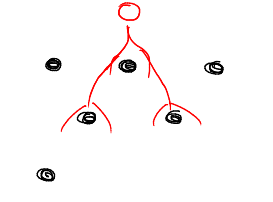
\includegraphics{fig1.png}
\end{figure}
\item \emph{Brownsche Bewegung}

\begin{figure}[h]
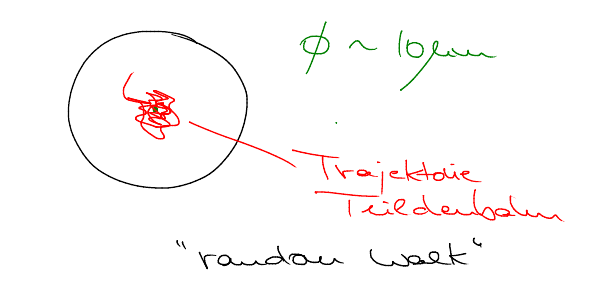
\includegraphics[scale=0.5]{fig2.png}
\end{figure}

\item \emph{Quantenmechanik}\\
Es gilt die Heisenbergsche Unschärferelation:
\[
\underbrace{\Delta x}_{\text{Ortsunschärfe}} \cdot \underbrace{\Delta p}_{\text{Impulsunschärfe}}
\]
\begin{figure}[h]
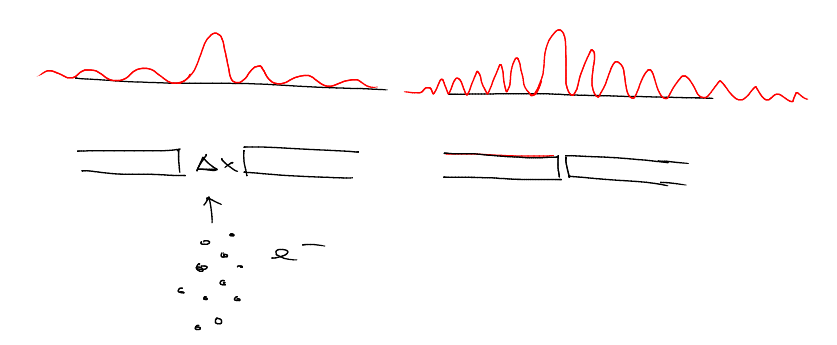
\includegraphics[scale=0.5]{fig3.png}
\end{figure}
\end{itemize}
\section{Physikalische Größen}
Eine \emph{Physikalische Größe} besteht aus einem \emph{Zahlenwert} und einer \emph{Einheit}.
\begin{ex*}
$1 \text{ in } \hat = \text{ Breite d. Daumens}$
Dies wurde später dann modifiziert, sodass die Einheit zur Länge drei aneinander liegenden Gerstenkörner umdefiniert worden ist.
\begin{figure}[h]
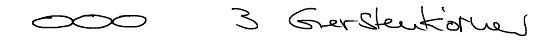
\includegraphics[scale=0.5]{fig4.png}
 \end{figure}
 
 Wünsche: wenige, aber überall nachprüfbare Einheiten $\rightarrow$ Basiseinheiten, Grundeinheiten
 \end{ex*}
 \end{seg}
 \subsection{Basiseinheiten}
 \begin{enumerate}[a]
\item Zeit \\
Die Grundeinheit der Zeit ist $1$ Sekunde(s).  Diese lässt sich definieren durch den Vergleich mit periodischen Vorgang. Es gilt:
\[
T=2\pi \sqrt{\frac{l}{g}}
\]

\[
l=24,8 \text{cm} \rightarrow T=1s
\]
\begin{itemize}
\item Quarzplättchen besitzen eine Frequenz aus dem $kHz$-Bereich.
\begin{figure}[h]
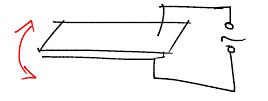
\includegraphics[scale=0.5]{fig5.png}
\end{figure}

Sie Besitzen einen Gangungenauigkeit von $1$ s/Woche. Sie besitzen also einen Fehler von $1$ s pro $10^6$ s
\item Es gibt aber auch die Möglichkeit mittels atomarer Eigenschwingungen (atomare Uhren) die Zeit noch genauer zu messen.  Deren Ganggenauigkeit entspricht $1$ s/$3000$ Jahren. Dies findet unter anderem Anwendung im GPS. 
\end{itemize}
\end{enumerate}
\end{document}
